%--------------------------------------
% Post Control Script Societies presentation
%--------------------------------------

\documentclass[aspectratio=169,xcolor=dvipsnames]{beamer}
\makeatletter
\def\input@path{{theme/}}
\makeatother
\usetheme{ICPHILCOMP25}
\usepackage{fix-cm}
\usepackage{amsmath}
\usepackage{mathtools}
\usepackage{listings}
\usepackage{xcolor}
\usepackage{hyperref}
\usepackage{graphicx}
\usepackage{tikz}
\usetikzlibrary{shapes.geometric, arrows.meta, positioning, fit, backgrounds}
\usepackage{etoolbox}

% Configure code listings
\lstset{
  basicstyle=\ttfamily\small,
  keywordstyle=\color{blue},
  commentstyle=\color{green!60!black},
  stringstyle=\color{red},
  showstringspaces=false,
  breaklines=true,
  frame=single,
  rulecolor=\color{black!30},
  backgroundcolor=\color{black!5},
  numbers=left,
  numberstyle=\tiny\color{black!70},
  numbersep=5pt
}

\title[Post Control Script Societies]{Post Control Script Societies}

\subtitle{Dinámicas de poder social mediante mecanismos de atención como inferencia activa.}

\author[Laura I. Rodríguez Dimayuga]{Laura I. Rodríguez Dimayuga}

\date{11 octubre 2026}

\titlegraphic{\colorbox{black}{
\includegraphics[height=1.5cm]{speaker_resources/philcomp_logo_white.png}}}



\begin{document}

\begin{frame}[plain]
  \titlepage
\end{frame}

\begin{frame}{Inferencia Activa(Active inference)}
  \begin{columns}[c]
    \begin{column}{0.48\textwidth}
La inferencia activa es una forma de comprender el comportamiento de los seres sintientes: una teoría que caracteriza la percepción, la planificación y la acción en términos de inferencia probabilística.\cite{parr2022active}
    \end{column}
    \begin{column}{0.42\textwidth}
      \centering
      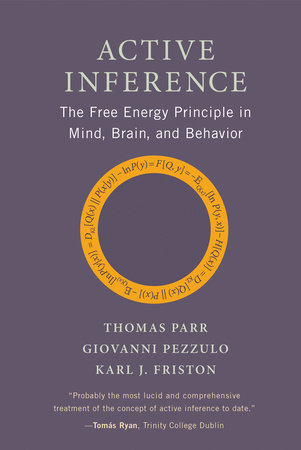
\includegraphics[height=0.68\textheight]{speaker_resources/active-inference.jpeg}
    \end{column}
  \end{columns}
\end{frame}

\begin{frame}
    \begin{columns}[c]
        \begin{column}{0.48\textwidth}
        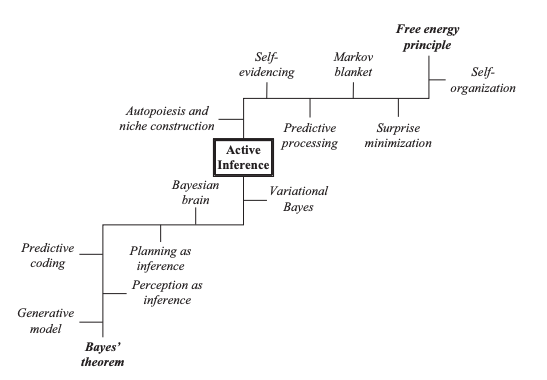
\includegraphics[width=0.9\textwidth]{speaker_resources/ai-bayesmap.png} \hfill 
        %\\ La vía de acceso directa a la inferencia activa parte de la noción del cerebro bayesiano, que concibe el cerebro como un motor de inferencia que intenta optimizar las representaciones probabilísticas de las causas de su entrada sensorial.
        \end{column}
        \begin{column}{0.48\textwidth}
            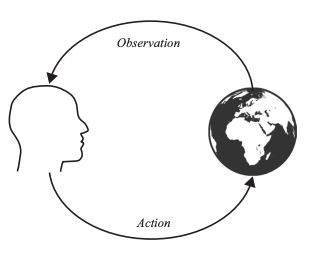
\includegraphics[width=0.9\textwidth]{speaker_resources/observation-action.png} \hfill 
        %\\ lo que los organismos vivos deben hacer para afrontar sus desafíos existenciales fundamentales (minimizar su energía libre) y por qué (para minimizar indirectamente la sorpresa de sus observaciones sensoriales) \cite{parr2022active}
        \end{column}
    \end{columns}
\end{frame}
\begin{frame}{Principio de Energía Libre (Free Energy Principle, FEP)}
  \begin{columns}[T,onlytextwidth]
    \begin{column}{0.56\textwidth}
      \small
    El cerebro reduce la sorpresa o la incertidumbre generando predicciones basadas en modelos internos y utiliza la información sensorial para actualizar dichos modelos, mejorando así la precisión de sus predicciones.

      \medskip
      Este principio supone una integración de la inferencia bayesiana y la inferencia activa, en la que la retroalimentación sensorial refina las acciones guiadas por predicciones. 
    \end{column}
    \begin{column}{0.38\textwidth}
      \centering
      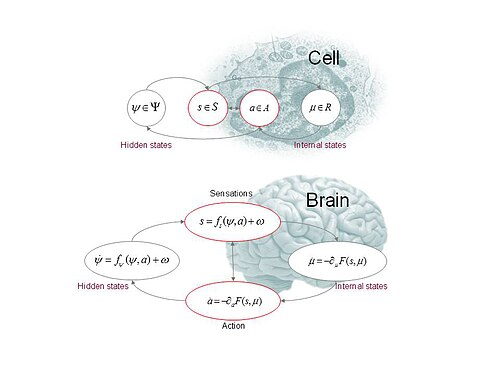
\includegraphics[width=\linewidth]{speaker_resources/fep.jpg}
    \end{column}
  \end{columns}
  \vfill
  \scriptsize Source: \url{https://en.wikipedia.org/wiki/Free_energy_principle}
\end{frame}

\begin{frame}{Funciones}
  \begin{columns}[T,onlytextwidth]
    \begin{column}{0.56\textwidth}
      \textbf{Función biológica.} La función biológica según Michael Levin va más allá de la simple ejecución genética o mecánica. Para él, la función biológica se entiende a través de la cognición colectiva y el código bioeléctrico.

      \medskip
      Una \textbf{función social} (como coordinar la confianza, pagar una deuda o saludarse) no depende de un individuo concreto. \textbf{Pasa a través} de los cuerpos mediante hábitos, palabras o monedas.

    \end{column}
    \begin{column}{0.38\textwidth}
      \begin{figure}
        \centering
        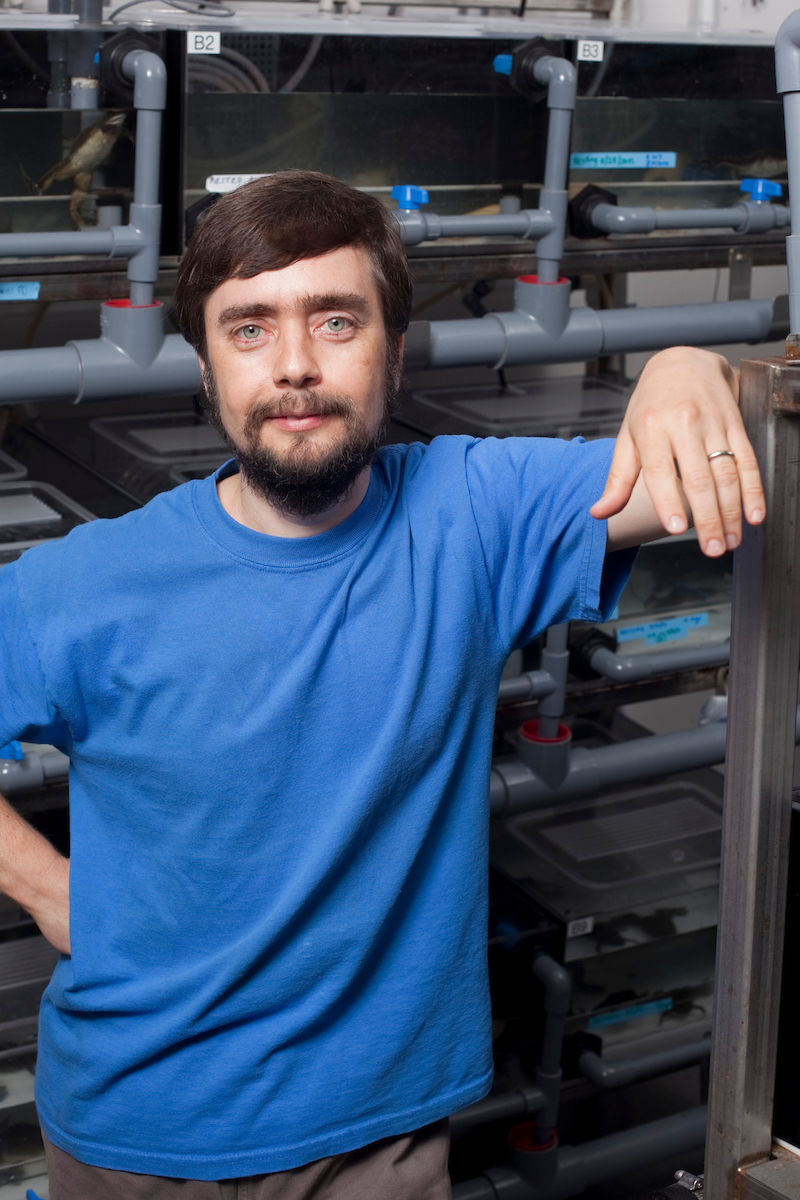
\includegraphics[width=0.6\linewidth]{speaker_resources/michael-levin.jpg}
      \end{figure}
    \end{column}
  \end{columns}
\end{frame}

\begin{frame}
    En ambos casos, se establece una relación cibernética entre el sistema y su entorno, donde la función no depende del sustrato material sino de la relación entre el sistema y su entorno.
    \medskip \\
    Kauffman y Clayton (2006): En ese artículo, los autores argumentan contra el reduccionismo radical y defienden que la agencia biológica mínima (minimal autonomous agency) emerge de la propia autoorganización termodinámica de un sistema (un sistema físico fuera del equilibrio que realiza al menos un ciclo de trabajo y reproduce sus propias condiciones de existencia).
    \medskip \\
    La \textbf{agencia} no requieren necesariamente una mente consciente humana previa ni una entidad fija, es una propiedad emergente de sistemas organizados que actúan para mantener su integridad y viabilidad frente a la entropía. 
\end{frame}
\begin{frame}
    \begin{figure}
        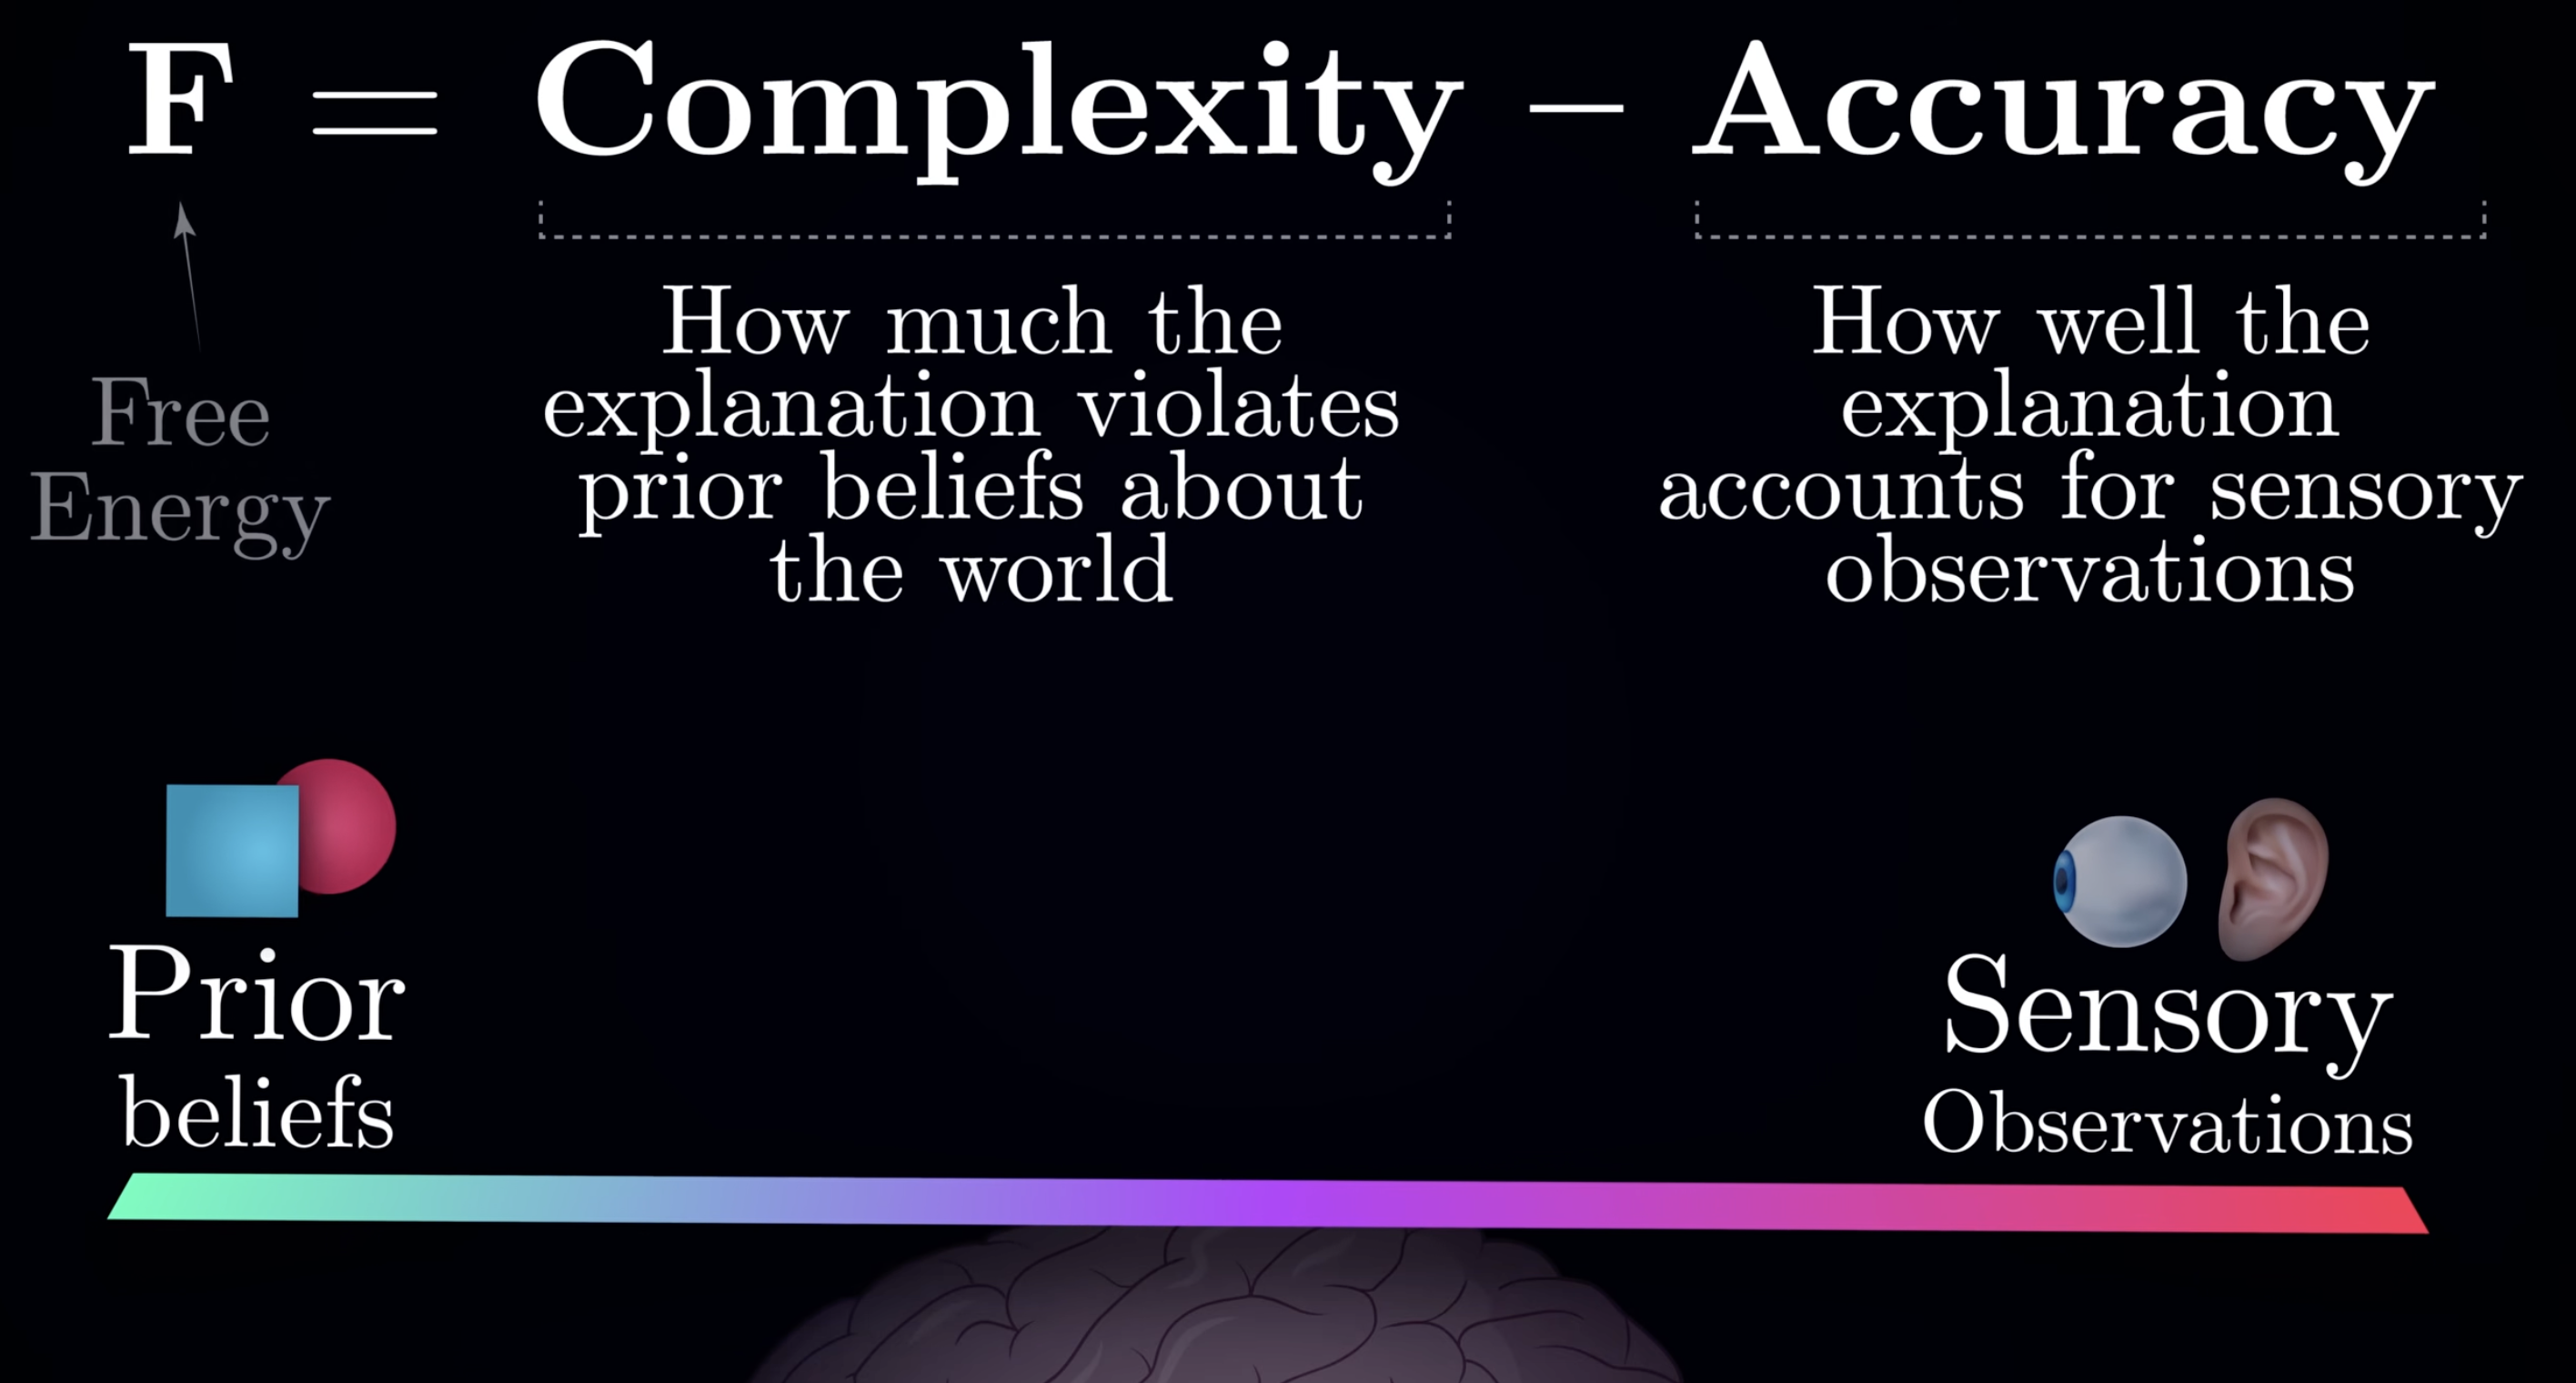
\includegraphics[width=0.8\linewidth]{speaker_resources/fepF.png}
    \end{figure}
\end{frame}
\begin{frame}{Enactivismo Computacional}
    \begin{columns}[T,onlytextwidth]
        \begin{column}{0.56\textwidth}
        \small
        El enactivismo computacional es un enfoque que combina la teoría enactivista de la mente con la computación, proponiendo que la cognición surge de la interacción dinámica entre un organismo y su entorno (FEP). 
        
        \medskip
        \textbf{Implicaciones:} los sistemas cognitivos  procesan información para responder a su ambiente, para ello utilizan 
        un modelo bayesiano, este es computable, ergo el enactivismo computacional es una forma de implementar el FEP en sistemas artificiales. \cite{korbak2021computational}
        \end{column}
        \begin{column}{0.38\textwidth}
        \centering
        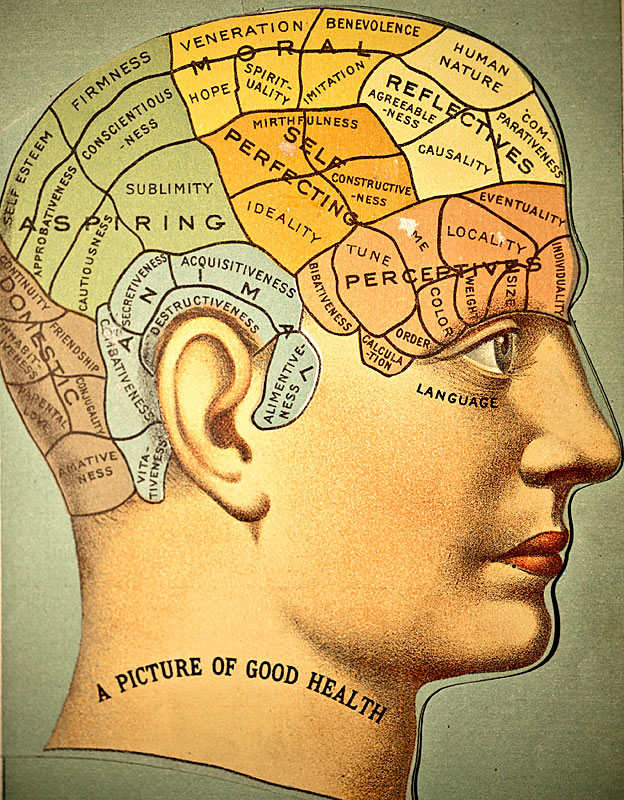
\includegraphics[width=0.8\linewidth]{speaker_resources/cerebro-dividido.jpg}
        \end{column}
    \end{columns}
\end{frame}

\begin{frame}{Definiciones de Poder}
    \begin{itemize}
    \item \textbf{Max Weber} definió el poder como la probabilidad de que un actor imponga su voluntad en una relación social, incluso frente a la resistencia (1978)
    \item \textbf{Hannah Arendt} el poder como una capacidad colectiva que surge cuando las personas actúan de manera concertada (coordinada). El poder no reside en individuos aislados, sino en la acción conjunta y la cooperación entre ellos (1970,1958)
    \item \textbf{Steven Lukes} El poder opera mediante la configuración de agendas (impidiendo la controversia) y, sobre todo, mediante la manipulación de percepciones y preferencias para que las posibles quejas nunca se materialicen (2005)
    \end{itemize}
\end{frame}
\begin{frame}
    \begin{itemize}
    \item \textbf{Antonio Gramsci} El poder se manifiesta en la hegemonía cultural, donde las ideas y valores dominantes moldean la percepción de la realidad y legitiman la autoridad de ciertos grupos sobre otros (1971)
    \item \textbf{Pierre Bourdieu} El poder simbólico opera a través del \textit{habitus}, la \textit{doxa} y el capital (económico, social, cultural, simbólico), de modo que las jerarquías persisten como el orden «natural» encarnado en la práctica y el reconocimiento.

    \item  \textbf{Michael Foucault} El poder se ejerce a través de redes de relaciones sociales, donde el conocimiento y la verdad son instrumentos de control y disciplina, organizando la atención mediante el control de la información (1975). 
    \end{itemize}
\end{frame}
\begin{frame}{Scripts(poder computacional)}
    El  poder no es una cosa, si no que las reglas de tranformación (dinámicas de relaciones) hace que lo podemos tratar como una \textbf{función}, un procesamiento de información, que transforma un estado de cosas en otro, y que puede ser implementado en un sistema computacional ... atráves de \textit{scripts}(programas-dispositivos de poder instanciados). 
    
    \begin{itemize}
        \item Transformando la modulazión de la atención en un mecanismo de control social. 
        \item Reforzando los patrones establecidos por los procesos de información. (La hegemonía de la información)
        \item El \textit{empoderamiento} se puede ver como la planeación probabilística computacional de predecir el futuro. (Machine Learning)
        \item Esto aplica en relaciones individuales (agente-agente) o 
        colectivas (agente-sociedad), atráves de \textit{atractores semánticos}(semantic attractors). 
    \end{itemize}
\end{frame}

\begin{frame}{Economía de la atención}
    Mediante estas estrategias, el poder puede movilizar cuerpos para reproducir condiciones materiales que refuerzan aún más las posiciones de poder existentes dentro de la economía social, atencional e informacional. \cite{wiki:economia_atencion}
    \begin{itemize}
        \item Ante la sobreabundancia de información, la atención se convierte en un recurso escaso y valioso, y el poder se ejerce a través de la capacidad de captar y dirigir esa atención.
        \item Debido a que la capacidad mental de los individuos es limitada, la atención se convierte en un recurso escaso y valioso. 
        \item Atráves del UX y la UI, se estudia cómo caputurar la atención de los usuarios y cómo dirigirla hacia ciertos contenidos o acciones deseadas.
    \end{itemize}
\end{frame}
\begin{frame}
    \begin{figure}
      \centering
      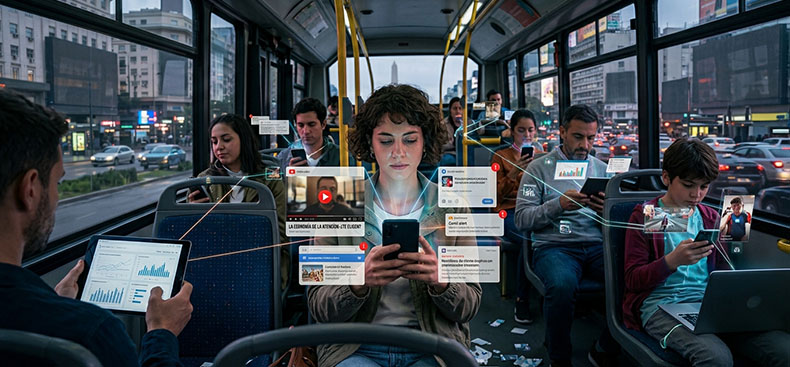
\includegraphics[width=0.9\textwidth]{speaker_resources/la-economia-de-la-atencion.jpg}
      \caption{La economía de la atención.}
    \end{figure}
\end{frame}
{\setbeamercolor{background canvas}{bg=black}
\begin{frame}[plain]
  \centering
  \resizebox{\textwidth}{!}{%
    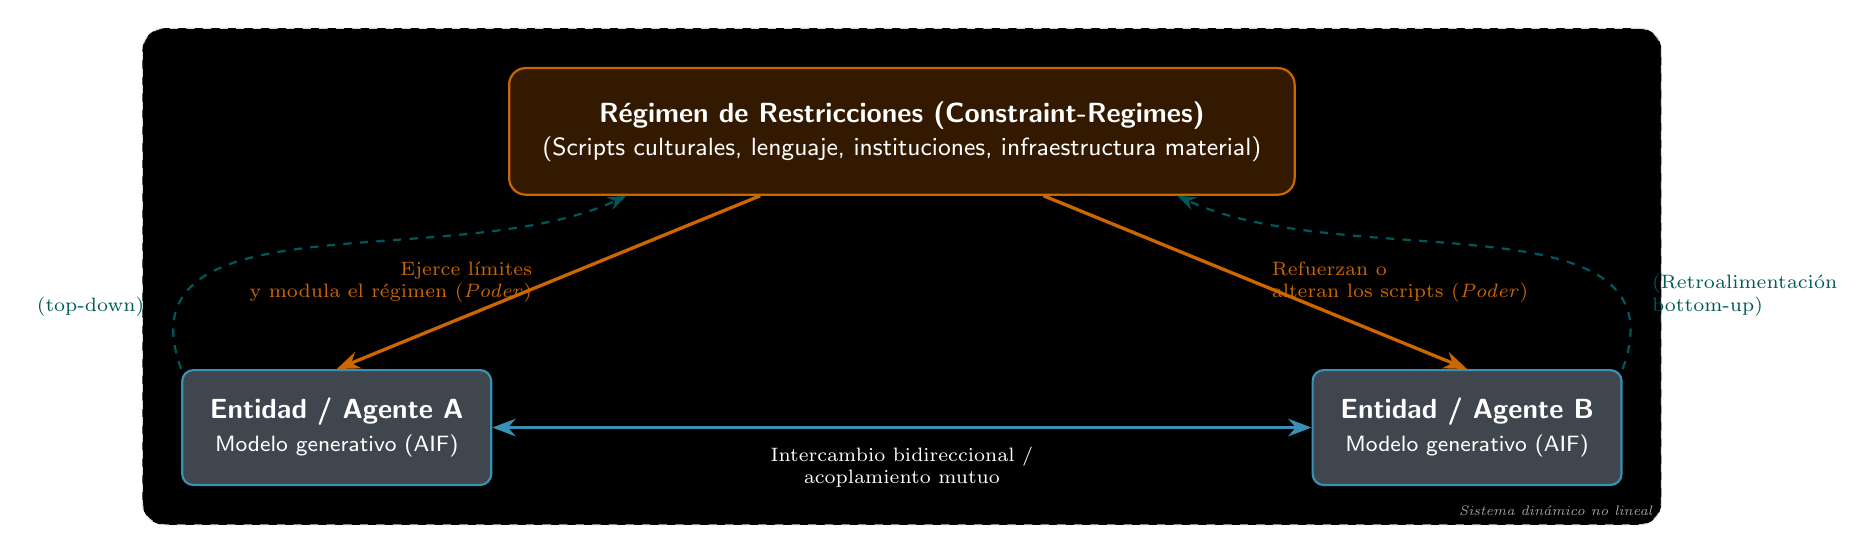
\begin{tikzpicture}[
    >=Stealth,
    font=\sffamily,
    node distance=1.8cm and 2.5cm,
    % Estilo de las cajas de entidades
    entity/.style={
        rectangle,
        rounded corners=4pt,
        draw=cyan!70!black,
        fill=cyan!20!black,
        text=white,
        thick,
        align=center,
        inner sep=10pt,
        minimum width=3.8cm,
        minimum height=1.4cm
    },
    % Estilo del régimen de restricciones
    regime/.style={
        rectangle,
        rounded corners=6pt,
        draw=orange!80!black,
        fill=orange!20!black,
        text=white,
        thick,
        align=center,
        inner sep=12pt,
        minimum width=9.5cm
    },
    % Estilos de líneas
    downward/.style={->, very thick, color=orange!80!black},
    upward/.style={->, thick, dashed, color=teal!70!black},
    mutual/.style={<->, very thick, color=cyan!70!black}
]

    % Régimen de restricciones (nivel superior)
    \node[regime] (CR) {
        \textbf{Régimen de Restricciones (\textit{Constraint-Regimes})} \\
        \small (Scripts culturales, lenguaje, instituciones, infraestructura material)
    };

    % Entidades / Agentes (nivel inferior)
    \node[entity, below left=2.2cm and 0.2cm of CR] (EA) {
        \textbf{Entidad / Agente A} \\
        \footnotesize Modelo generativo (AIF)
    };
    
    \node[entity, below right=2.2cm and 0.2cm of CR] (EB) {
        \textbf{Entidad / Agente B} \\
        \footnotesize Modelo generativo (AIF)
    };

    % 1. Interacción horizontal (multidireccional entre agentes)
    \draw[mutual] (EA) -- (EB) 
        node[midway, below=3pt, align=center, font=\scriptsize, text=white] {
            Intercambio bidireccional /\\
            acoplamiento mutuo
        };

    % 2. Influencia vertical descendente (Top-down: constriñe y modula)
    \draw[downward] ([xshift=-1.8cm]CR.south) -- (EA.north)
        node[midway, left=2pt, align=right, font=\scriptsize, text=orange!80!black] {
            Ejerce límites \\ y modula el régimen (\textit{Poder})
        };
        
    \draw[downward] ([xshift=1.8cm]CR.south) -- (EB.north)
        node[midway, right=2pt, align=left, font=\scriptsize, text=orange!80!black] {
            Refuerzan o \\ alteran los scripts (\textit{Poder})
        };

    % 3. Influencia vertical ascendente / retroactiva (Bottom-up: sedimentación o cambio)
    \draw[upward] (EA.north west) to[out=110, in=205] ([xshift=-3.5cm]CR.south)
        ;
    \node[anchor=south east, xshift=-0.25cm, yshift=0.55cm,
        align=right, font=\scriptsize, text=teal!70!black] at (EA.north west) {
        (top-down)
    };

    \draw[upward] (EB.north east) to[out=70, in=335] ([xshift=3.5cm]CR.south)
        ;
    \node[anchor=south west, xshift=0.25cm, yshift=0.55cm,
        align=left, font=\scriptsize, text=teal!70!black] at (EB.north east) {
        (Retroalimentación \\ bottom-up)
    };

    % Fondo que enmarca la totalidad como un sistema interactivo
    \begin{scope}[on background layer]
        \node[
            draw=gray!30,
            dashed,
            rounded corners=8pt,
            fill=black,
            fit=(CR) (EA) (EB),
            inner sep=14pt,
            label={[anchor=south east, font=\itshape\tiny, text=gray!70]south east:Sistema dinámico no lineal}
        ] {};
    \end{scope}

\end{tikzpicture}%
  }
\end{frame}}

\begin{frame}{Biopólitica (Foucault)}
    Gestión, regualción y optimización de la vida. 
    \begin{itemize}
        \item Políticas de la salud pública, educación, urbanismo, seguridad, etc. 
        \begin{itemize}
            \item Constituyen \textit{scripts} institucionales compartidos que sincronizan expectativas y minimizan la incertidumbre colectiva, definiendo qué conductas higiénicas se consideran normales o transgresoras.
        \end{itemize}
    \end{itemize}
    \begin{figure}
        \centering
        
\includegraphics[width=0.5\textwidth]{speaker_resources/vacunas.jpg}
    \end{figure}
\end{frame}

\begin{frame}
    \frametitle{Control poblacional, demográfico y de la natalidad}
    \begin{itemize}
        \item Funcionan como atractores semánticos y presunciones  de alto peso (precision-weighting / prior-bayes) que internalizan las prioridades del Estado en las decisiones corporales íntimas.
    \end{itemize}
    \begin{figure}
        \centering
        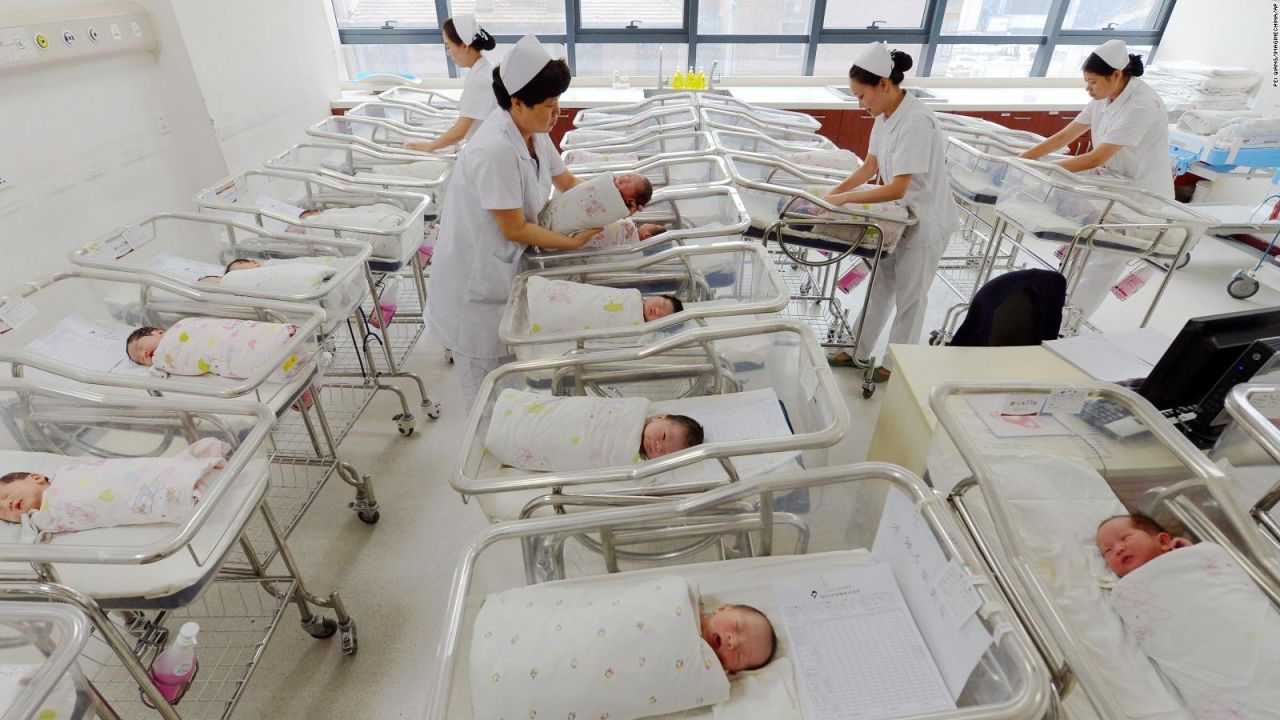
\includegraphics[width=0.5\textwidth]{speaker_resources/natalidad.jpg}
    \end{figure}
\end{frame}

\begin{frame}
    \frametitle{Sistemas de identificación biométrica y vigilancia dispersa}
  \begin{columns}[T,onlytextwidth]
    \begin{column}{0.56\textwidth}
      \begin{itemize}
        \item Representa el paso de los encierros disciplinarios físicos (cárceles, fábricas) a las sociedades de control donde el panóptico se disemina en la infraestructura tecnológica. El control ya no requiere muros constantes; basta con la modulación atencional y el registro continuo de datos que aseguran la predictibilidad del sujeto.
      \end{itemize}
    \end{column}
    \begin{column}{0.38\textwidth}
      \begin{figure}
        \centering
        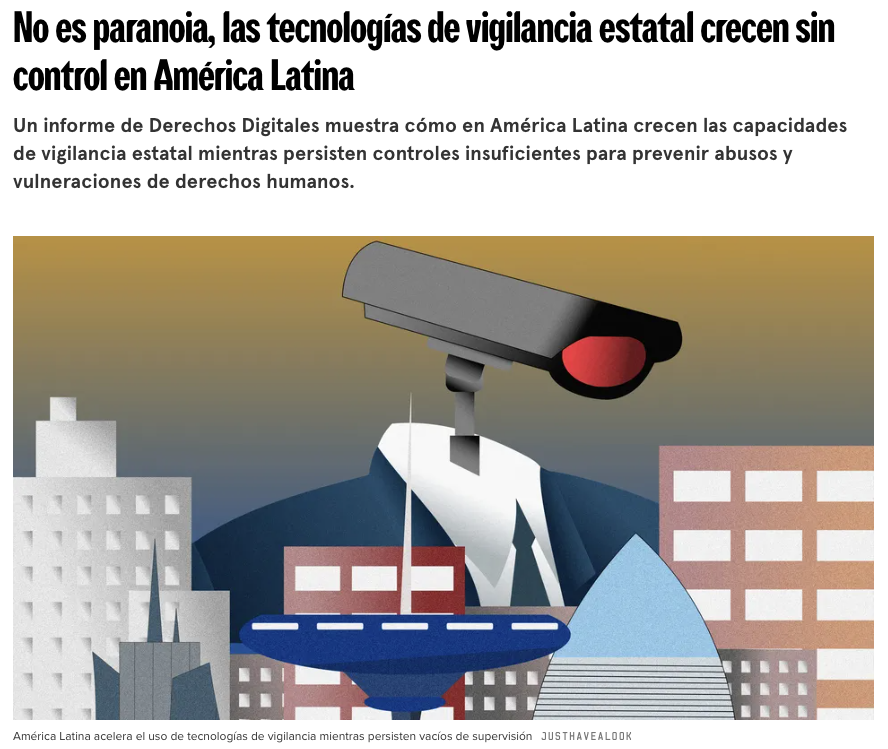
\includegraphics[width=\linewidth]{speaker_resources/vigilancia.png}
        \caption{Fuente. Aranza Bustamante, \textit{No es paranoia, las tecnologías de vigilancia estatal crecen sin control en América Latina}, 5 de octubre 2026.}
      \end{figure}
    \end{column}
  \end{columns}
\end{frame}

\begin{frame}{La modulazión}

    \begin{itemize}
        \item La modulazión distribuida. 
        \item El ajuste de los parámetros de atención y precisión en los modelos generativos de los agentes
        \item La modulación reduce la incertidumbre y la sorpresa, y por lo tanto la energía libre, al guiar el comportamiento de los agentes hacia estados más predecibles y estables.
        \item Tomando ideas de Gilbert Simondon y Yuk Hui, modular no es imponer una forma sobre la materia de manera estática, sino una auto-regulación continua donde se alteran gradualmente las frecuencias y restricciones que orientan la vida en común.
    \end{itemize}
    \iffalse
    El poder opera como una gestión de flujos o modulación distribuida, no residen en un único centro de mando, individuo o institución soberana, sino que emergen y operan a través de toda la red de relaciones, prácticas, tecnologías y hábitos compartidos.

    La atención se formaliza como la modulación de la precisión (), es decir, el ajuste de la confianza o el peso que el cerebro asigna a determinadas señales sensoriales, creencias previas o predicciones de políticas de acción.

    En lugar de forzar físicamente a un individuo (lo que requiere un gasto energético constante de control directo), la modulación altera el entorno, los incentivos o el modelo generativo del sujeto para que este elija voluntariamente la conducta esperada, minimizando su propia incertidumbre o energía libre. 

    Tomando ideas de Gilbert Simondon y Yuk Hui, modular no es imponer una forma sobre la materia de manera estática, sino una auto-regulación continua donde se alteran gradualmente las frecuencias y restricciones que orientan la vida en común
    \fi
\end{frame}

\begin{frame}{Atractores Sémanticos}
  \begin{columns}[T,onlytextwidth]
    \begin{column}{0.56\textwidth}
      \begin{itemize}
        \item Un atractor es un estado o conjunto de estados hacia el cual un sistema tiende a evolucionar de manera natural a lo largo del tiempo. (ejemplo: una bola rodando hacia el fondo de un valle)
        \item En una situación social o comunicativa ambigua, tu cerebro no se queda flotando en el vacío ni calcula infinitas posibilidades; rápidamente «cae» en un significado concreto y familiar (el atractor).
        \item La atracción hacia la satisfacción del deseo
      \end{itemize}
    \end{column}
    \begin{column}{0.38\textwidth}
      \begin{figure}
        \centering
        
\includegraphics[width=\linewidth]{speaker_resources/atractor.jpg}
        \caption{Sistemas dinámicos y atractores.}
      \end{figure}
    \end{column}
  \end{columns}
\end{frame}

\begin{frame}{Conclusiones}
    Pasamos de la idea de un control jeraquica a un script de carácter modulador. De ahí: post-script control societies.
    \bigskip
    La inferencia activa hace visibles las capas de scripts que controlan nuestra atención y elección. La autora nos invita a reflexionar sobre la distribución del poder de quién controla la información y los mecanismos de atención, y cómo esto afecta la autonomía individual y colectiva.
\end{frame}

\begin{frame}{Implicaciones}
    Cuando los scripts son internalizados, incorporados y organizados por múltiples miembros de una comunidad, esto permite la construcción colectiva de estados futuros.
    \bigskip
    Es importante reconocer los programas/algortimos que guían nuestras decisiones y acciones, y cómo estos scripts pueden ser diseñados para fomentar la cooperación, la equidad y el bienestar social. En lugar de dejar que sean escritos por intereses particulares, podemos participar en la creación de scripts que reflejen valores compartidos y promuevan un futuro más justo y sostenible.
\end{frame}

\begin{frame}{Preguntas}
   \begin{itemize}
    \item ¿Cómo podemos medir cuantitativamente el poder probabilistico de un script?
    \item ¿Cómo realizamos intervenciones o moficaciones en los scripts para fomentar la cooperación y la equidad?
    \item ¿Qué podemos rescatar de una perspectiva computacional de la filosofía política y social?
   \end{itemize} 
\end{frame}
\begin{frame}
    Los \textbf{scripts} funcionan como atractores semánticos: patrones compartidos que atraen la atención colectiva hacia interpretaciones predecibles, reduciendo la incertidumbre y el gasto cognitivo de interpretar la realidad desde cero.
\end{frame}
\begin{frame}[allowframebreaks]{Referencias}
  \bibliographystyle{plain}
  \bibliography{reference}
\end{frame}

\end{document}
